\documentclass{beamer}

\title{Mid-PhD Defense}
\author{Paul Dubois}
\institute{
	TheraPanacea\\
	MICS, CentraleSupélec\\
	Institut du Cancer de Montpellier
}
\date{21st June 2023}

\usepackage{tikz}

\begin{document}
	
	\frame{\titlepage}
	
	% problem def
	% fluence to bixels
	% DI matrix generation
	% cost func
	% optimizers comp' => ArXiV!!!
	% dose distance => Soon submitted?
	% dose clustering => Almost finished writing!
	% pareto appendix?
	% RL setup => normalization of constr; reward func
	% ccl
	
	\begin{frame}
		\frametitle{Automatic Dose Optimization for Radiotherapy}
		
		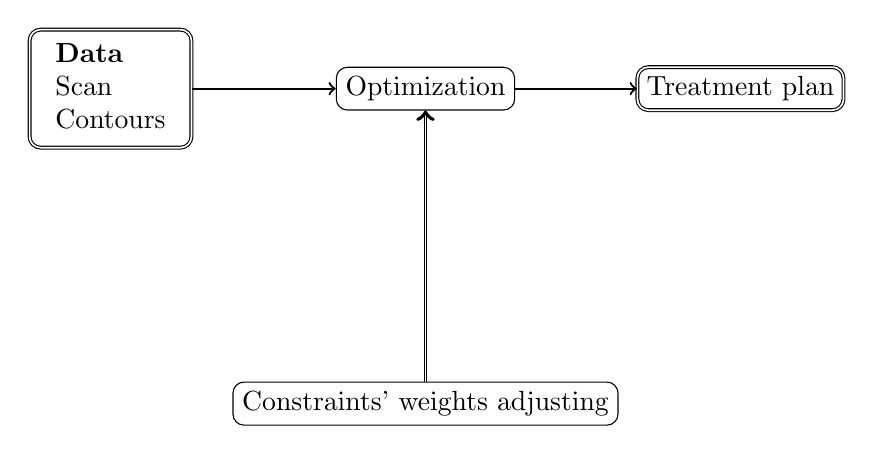
\begin{tikzpicture}[node distance=4cm]
			\node (inputs) [draw,double,rounded corners] {\begin{tabular}{l} \textbf{Data} \\ Scan \\ Contours \end{tabular}};
			\node (process) [right of=inputs,draw,rounded corners] {Optimization};
			\node (outputs) [right of=process,draw,double,rounded corners] {Treatment plan};
			
			\draw [thick,->] (inputs) -- (process);
			\draw [thick,->] (process) -- (outputs);
			
			\node (human) [,below of=process,draw,rounded corners] {Constraints' weights adjusting};
			
			\draw [double,<-] (process) -- (human);
			
		\end{tikzpicture}
		
	\end{frame}
	
	\begin{frame}
		\frametitle{Problem Formulation}
		\framesubtitle{IMRT}
		
		Bixel values:
		$$x_{i,j}^\theta \geq 0 \text{, for } \theta \in \Theta \text{ and } 1\leq i,j \leq 20\footnote{20x20 is a typical bixel discretization}$$
		usually concatenated to a single bixels-value vector $x$.
		\vspace{0.5cm}
		
		Dose calculation:
		$$\textbf{y} = L\textbf{x} \text{ with } L \text{ (pre-calculated) dose-influence (DI) matrix}$$
		
	\end{frame}
	
	\begin{frame}
		\frametitle{Problem Formulation}
		\framesubtitle{IMRT (bis)}
		
		Objective for \textit{maximum} constraint $c$ on structure $s$, dose $d$:
		$$f_c(\textbf{y}) = \frac{1}{|\mathcal{V}|} \sum_{v \in \mathcal{V}} (\textbf{y}_v-d)_+^2$$
		(reverse sign for minimal constraint).
		\vspace{0.5cm}
		
		Final objective:
		$$f(\textbf{y}) = \sum_{c \in \mathcal{C}} w_c f_c(\textbf{y})$$
		with $w_c$ the weight of constraint $c$.
		
	\end{frame}
	
	\begin{frame}
		\frametitle{Problem Optimization}
		\framesubtitle{Optimizer review}
				
		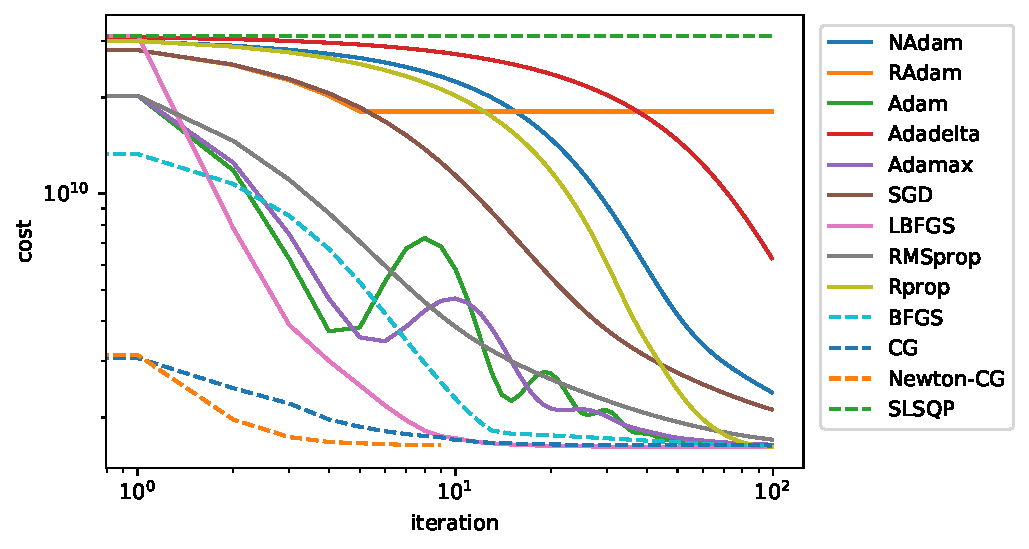
\includegraphics[width=11cm]{figures/ICMProstate-iter.pdf}
		
		\url{https://arxiv.org/abs/2305.18014}
		
	\end{frame}
	
	\begin{frame}
		\frametitle{Problem Optimization}
		\framesubtitle{Optimizer review (bis)}
		
		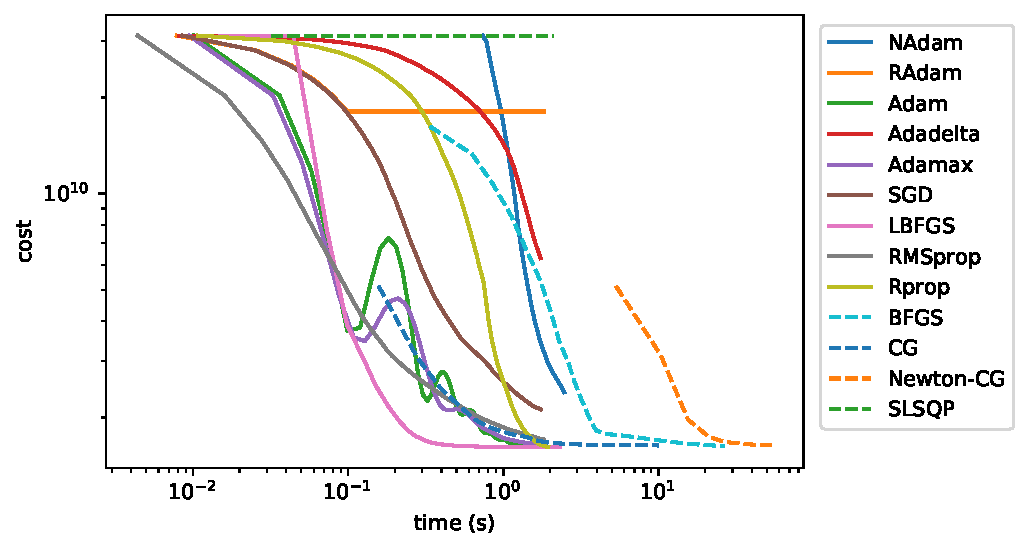
\includegraphics[width=11cm]{figures/ICMProstate-time.pdf}
		
		\url{https://arxiv.org/abs/2305.18014}
	
	\end{frame}
	
\end{document}